\documentclass[12pt]{article}
\usepackage{scrextend}
\usepackage[utf8]{inputenc}
\usepackage[polish]{babel}
\usepackage[T1]{fontenc}%polskie znaki
\usepackage[utf8]{inputenc}%polskie znaki
\usepackage{geometry}
\usepackage{float}
\usepackage{enumitem}
\usepackage{hyperref}
\usepackage{graphicx}
\usepackage{tabulary}
\usepackage{etoc}
\usepackage[normalem]{ulem} 
\renewcommand{\baselinestretch}{1.5}
\graphicspath{ {img/} }
\newgeometry{lmargin=2cm, rmargin=2cm, tmargin=2cm, bmargin=2cm}
\usepackage{tikz}
\usepackage[bf]{caption}
\usepackage{setspace}
\usepackage{rotating}
\newcommand{\scenario}[5]{
  \subsection{#1}
  \begin{minipage}{\textwidth}
    \textbf{Cel:} #2 \\
    \textbf{WS:} #3 \\
    \textbf{WK:} #4 \\
    \textbf{Przebieg:}
    \begin{enumerate}
      \setlength\itemsep{0.0em}
      #5
    \end{enumerate}
  \end{minipage}
}
\hyphenation{include}
\hyphenation{extend}



\usepackage{listings}
\usepackage{xcolor}
 
\definecolor{codegreen}{rgb}{0,0.6,0}
\definecolor{codegray}{rgb}{0.5,0.5,0.5}
\definecolor{codepurple}{rgb}{0.58,0,0.82}
\definecolor{backcolour}{rgb}{0.99,0.99,0.973}
 
\lstdefinestyle{mystyle}{
    backgroundcolor=\color{backcolour},   
    commentstyle=\color{codegreen},
    keywordstyle=\color{magenta},
    numberstyle=\tiny\color{codegray},
    stringstyle=\color{codepurple},
    basicstyle=\ttfamily\footnotesize,
    breakatwhitespace=false,         
    breaklines=true,                 
    captionpos=b,                    
    keepspaces=true,                 
    numbers=left,                    
    numbersep=5pt,                  
    showspaces=false,                
    showstringspaces=false,
    showtabs=false,                  
    tabsize=2
}
\lstset{
    extendedchars=false,
    inputencoding=utf8
}
\renewcommand{\lstlistlistingname}{Spis listingów}\lstset{style=mystyle}


\begin{document}

\begin{flushleft}
    Damian Koper, \textbf{241292} \\
    Łukasz Handschuh, \textbf{241402}
\end{flushleft}
\vspace{1cm}
{
\centering
{\Huge\scshape\bfseries Inżynieria oprogramowania - Etap 5 }\\
\vspace{0.25cm}
\Large\textbf{Dział ewidencji ludności} \\
\vspace{0.25cm}
\large Opracowanie diagramów stanów dla wybranych klas,
reprezentujących wpływy różnych przypadków użycia na
zmiany stanów tych klas, modelowanych za pomocą
diagramów sekwencji.\\
}

\begin{figure}[H]
    \centering
        \makebox[0pt]{
    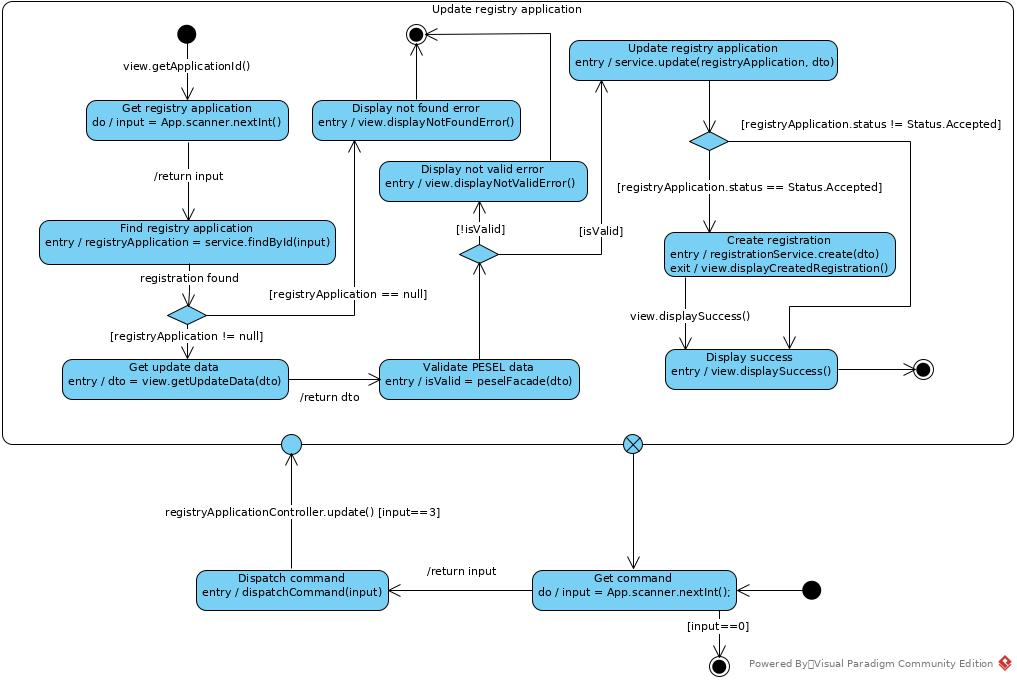
\includegraphics[
        keepaspectratio,
        width=1.1\linewidth,
        height=\dimexpr\textheight-9\baselineskip
    ]{./../paragidm/export/PopulationRegistry_STD_2.jpg}
    }
    \caption{Diagram stanów - aktualizowanie wniosków.}
    \label{}
\end{figure}
\clearpage
\begin{figure}[H]
    \centering
        \makebox[0pt]{
    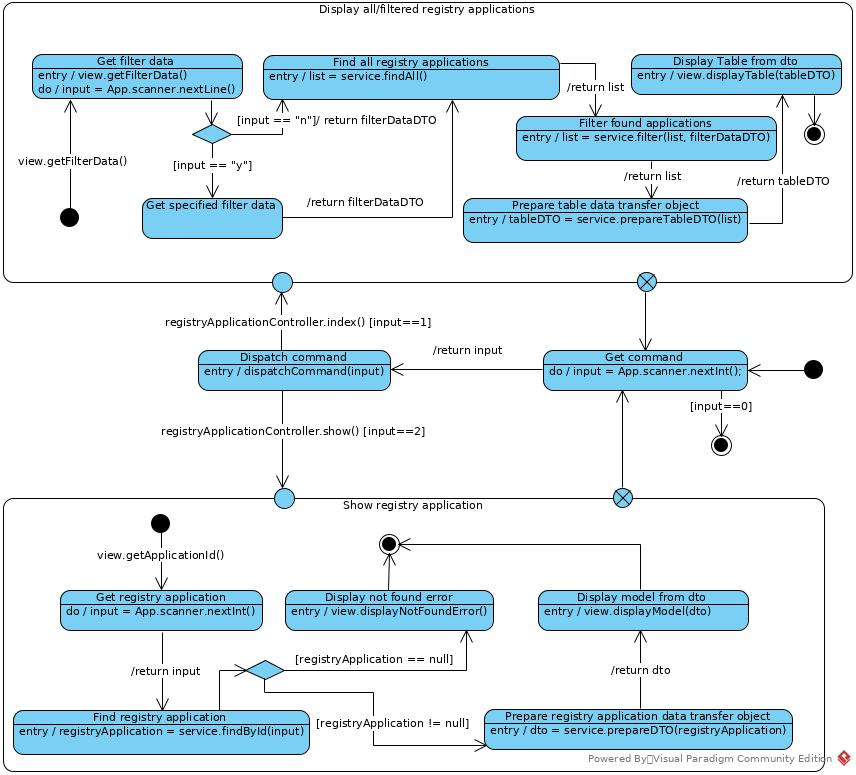
\includegraphics[
        keepaspectratio,
        width=1.1\linewidth,
        height=\dimexpr\textheight-9\baselineskip
    ]{./../paragidm/export/PopulationRegistry_STD_1.jpg}
    }
    \caption{Diagram stanów - wyświetlanie pojedynczego i wszystkich wniosków.}
    \label{}
\end{figure}

\end{document}
